\documentclass[12pt, letterpaper]{article}

% Font
\usepackage[utf8]{inputenc}
\usepackage{MinionPro} 
\input{glyphtounicode}
\pdfgentounicode=1 
\usepackage{microtype}

% Format
\usepackage[letterpaper, margin = 1in]{geometry}
\setcounter{secnumdepth}{0}
\usepackage{titlesec}  
\titleformat*{\section}{\centering\normalfont\Large\bfseries}

% Links
\usepackage[colorlinks = true, linkcolor = black, urlcolor = black, citecolor = black]{hyperref} 

% Figures
\usepackage{graphicx}
\usepackage[labelfont = bf, font = small, labelsep = newline, singlelinecheck = false]{caption}
\renewcommand{\thefigure}{S\arabic{figure}}

% Tables
\usepackage{booktabs}
\usepackage{tabularx}

% References
\newenvironment{CSLReferences}[2]{}{}

% Frontmatter
\title{ Supplemental Online Materials:\\\textit{Meta-Analysis of the
`Ironic' Effects of Intergroup Contact} }
\author{  }

\begin{document}

\maketitle

\hypertarget{search-strategy}{%
\subsection{Search Strategy}\label{search-strategy}}

We used similar non-exclusive search terms for all electronic databases:

\begin{enumerate}
\def\labelenumi{\arabic{enumi}.}
\item
  (contact OR friendship) AND (``perceived discrimination'' OR
  ``perceived *advantage'' OR ``relative deprivation'' OR ``group
  discrimination'' OR ``personal discrimination'' OR ``group
  deprivation'' OR ``perception* of discrimination'' OR ``perception* of
  group discrimination'' OR ``perception* of personal discrimination''
  OR ``rac* discrimination'')
\item
  *group AND (contact OR friendship) AND (``collective action'' OR
  protest OR ``collective behavio*r'' OR ``political behavio*r'' OR
  ``social change'' OR ``social justice'')
\item
  *group AND (contact OR friendship) AND (policy OR policies OR
  ``affirmative action'' OR (politi* W/15 attitude*) OR (politi* W/15
  preferenc*)) AND (redistribut* OR reparati* OR inequalit* OR equalit*
  OR injustice* OR justice* OR disadvantage* OR advantage* OR minorit*
  OR majorit*)
\end{enumerate}

\noindent We sent a call for unpublished research to the mailing lists
of the \emph{European Association of Social Psychology}, the
\emph{Society for Personality and Social Psychology}, the
\emph{International Society of Political Psychology}, the \emph{Society
for the Psychological Study of Social Issues}, and the \emph{Society of
Australasian Social Psychologists}.

\hypertarget{coding-criteria-study-setting}{%
\subsection{Coding Criteria (Study
Setting)}\label{coding-criteria-study-setting}}

For each sample, we categorized the study setting according to the
source of the ingroup's relative disadvantage. This coding scheme is, by
necessity, reductive and incomplete. We believe, however, that it can
offer some insight into relevant differences in study settings.

We coded a study setting as \emph{short-term migration} if the relevant
intergroup context resulted from the short-term movement of people for
the purposes of temporary employment or education. Most studies in this
category focus on international students.

We coded a study setting as \emph{long-term migration} if the relevant
intergroup context resulted from migration, in either the current or
previous generations, and if there is an established intergroup
hierarchy that disadvantages the relevant ingroup. Examples include
Black and Asian people in the United Kingdom and Asian Americans in the
United States.

We coded a study setting as \emph{post-slavery} if the ingroup's
relative disadvantage resulted from a racial hierarchy rooted in the
historical abduction and enslavement of Africans. This category includes
Black people in the Americas and the Caribbean.

We coded a study setting as \emph{colonization} if the relevant
intergroup context resulted from the advantaged group colonizing and
subjugating the disadvantaged group in the place that was originally
inhabited by the disadvantaged group. This category includes contexts in
which one nation has occupied the territory of another, resulting in an
established intergroup hierarchy that disadvantages the relevant
ingroup. Examples include Māori in New Zealand and Kurds in Turkey.
While many of the hierarchies we categorize as resulting from long-term
migration or slavery are rooted in a history of colonization, we use
colonization in a narrow sense to describe settler colonies and occupied
territories.

We coded a study setting as \emph{religion} if the relevant intergroup
context was defined in terms of religious group membership (for example,
Muslims in India). In contexts in which religion is a marker of a
disadvantaged immigrant group (e.g., Muslims in the Netherlands), we
instead categorized the study setting as long-term migration.

We coded a study setting as \emph{caste} if the ingroup's relative
disadvantaged resulted from caste hierarchies in South Asia. We coded a
study setting as \emph{sexual/gender minorities} if the relevant ingroup
was defined in terms of their membership in a discriminated sexual or
gender minority (i.e., LGBTQ people). We coded a study setting as
\emph{other} if the relevant intergroup context did not fit any of the
other categories (e.g., disabled people).

\hypertarget{moderator-analyses}{%
\subsection{Moderator Analyses}\label{moderator-analyses}}

First, we ran a series of Bayesian random-effects meta-regression models
to estimate how much of the between-samples heterogeneity was explained
by specific categorical moderator variables
(\texttt{run\_moderator\_analyses.R}). Figures S1 and S2 show the
results for collective action and policy support. Comparisons were
inconclusive because we had an insufficient number of effect sizes per
category.

Second, we ran another three random-effects meta-regression models with
Muthukrishna et al.'s (2020) measure of cultural distance, where
available, as a continuous moderator variable. Because cultural distance
was a country-level moderator variable, we used two-level random-effects
models in which we estimated country-specific deviations from the mean
effect size as well as sample-specific deviations from the
country-specific effect size. Figure 5 (in the main text) show the
inconclusive results for all three outcomes.

Third, we used meta-regression trees to discover interactions between
moderator variables that best explained heterogeneity in effect sizes
(Li et al., 2017). As recommended, we ran random-effects meta-regression
tree analyses using the look-ahead strategy (Li et al., 2020). We set
the pruning parameter to \(c = 0\) because, for this analysis, we
prioritized exploration over error control
(\texttt{run\_exploratory\_moderator\_analyses.R}). For both collective
action and policy support, the algorithm found that no moderator or
interaction of moderators explained between-samples heterogeneity. This
result is not surprising, however, as both analyses used fewer than 40
effect sizes, the minimum number required for the algorithm to perform
well in detecting even simple interaction effects (Li et al., 2017). As
all moderator analyses were inconclusive for collective action and
policy support, we only report results for perceived injustice in the
main text.

\begin{figure*}
\centering
\caption{Estimated effect sizes for the association between intergroup contact and collective action as a function of various categorical moderator variables}
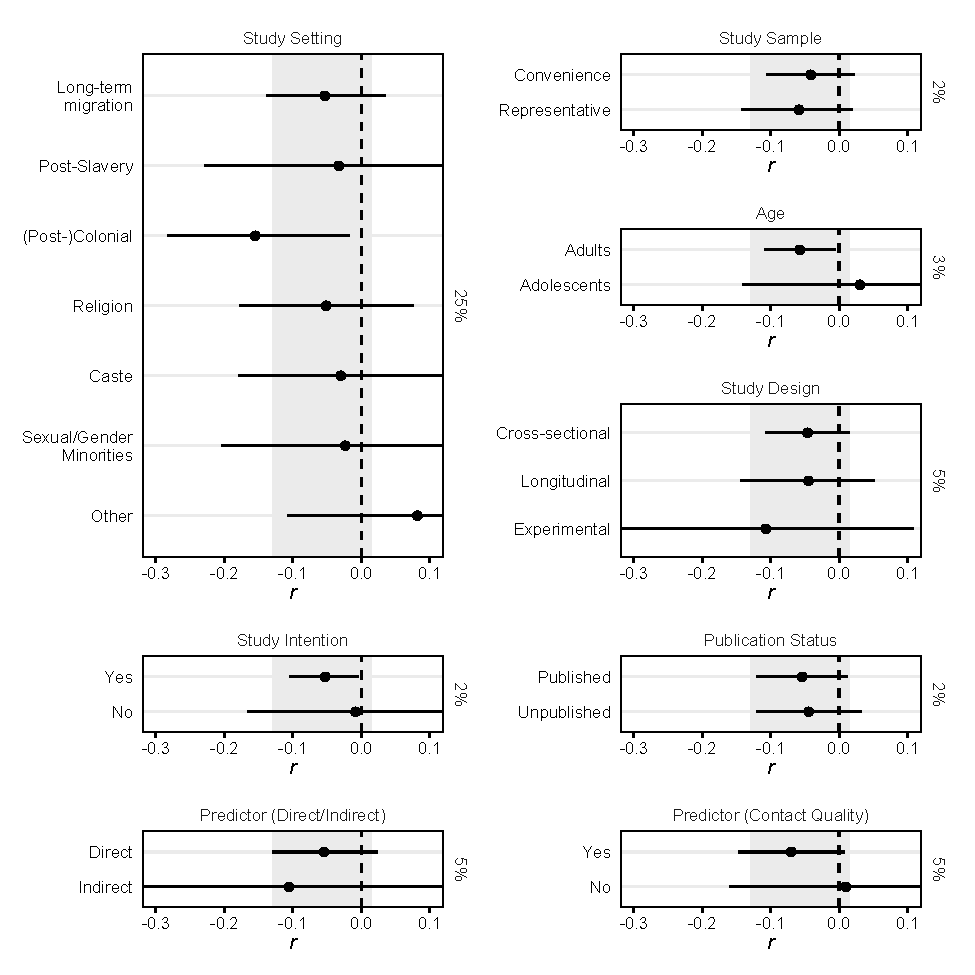
\includegraphics[scale=1]{../figures/figure-s1}
\caption*{\textit{Note.} Intervals enclose the 95\% most plausible estimates of the category-specific effect size. Shaded ribbons enclose the 95\% most plausible estimates of the mean effect size from the main analyses. Percentages indicate the estimated between-sample variance explained by each moderator variable.}
\label{fig:s1}
\end{figure*}

\begin{figure*}
\centering
\caption{Estimated effect sizes for the association between intergroup contact and policy support as a function of various categorical moderator variables}
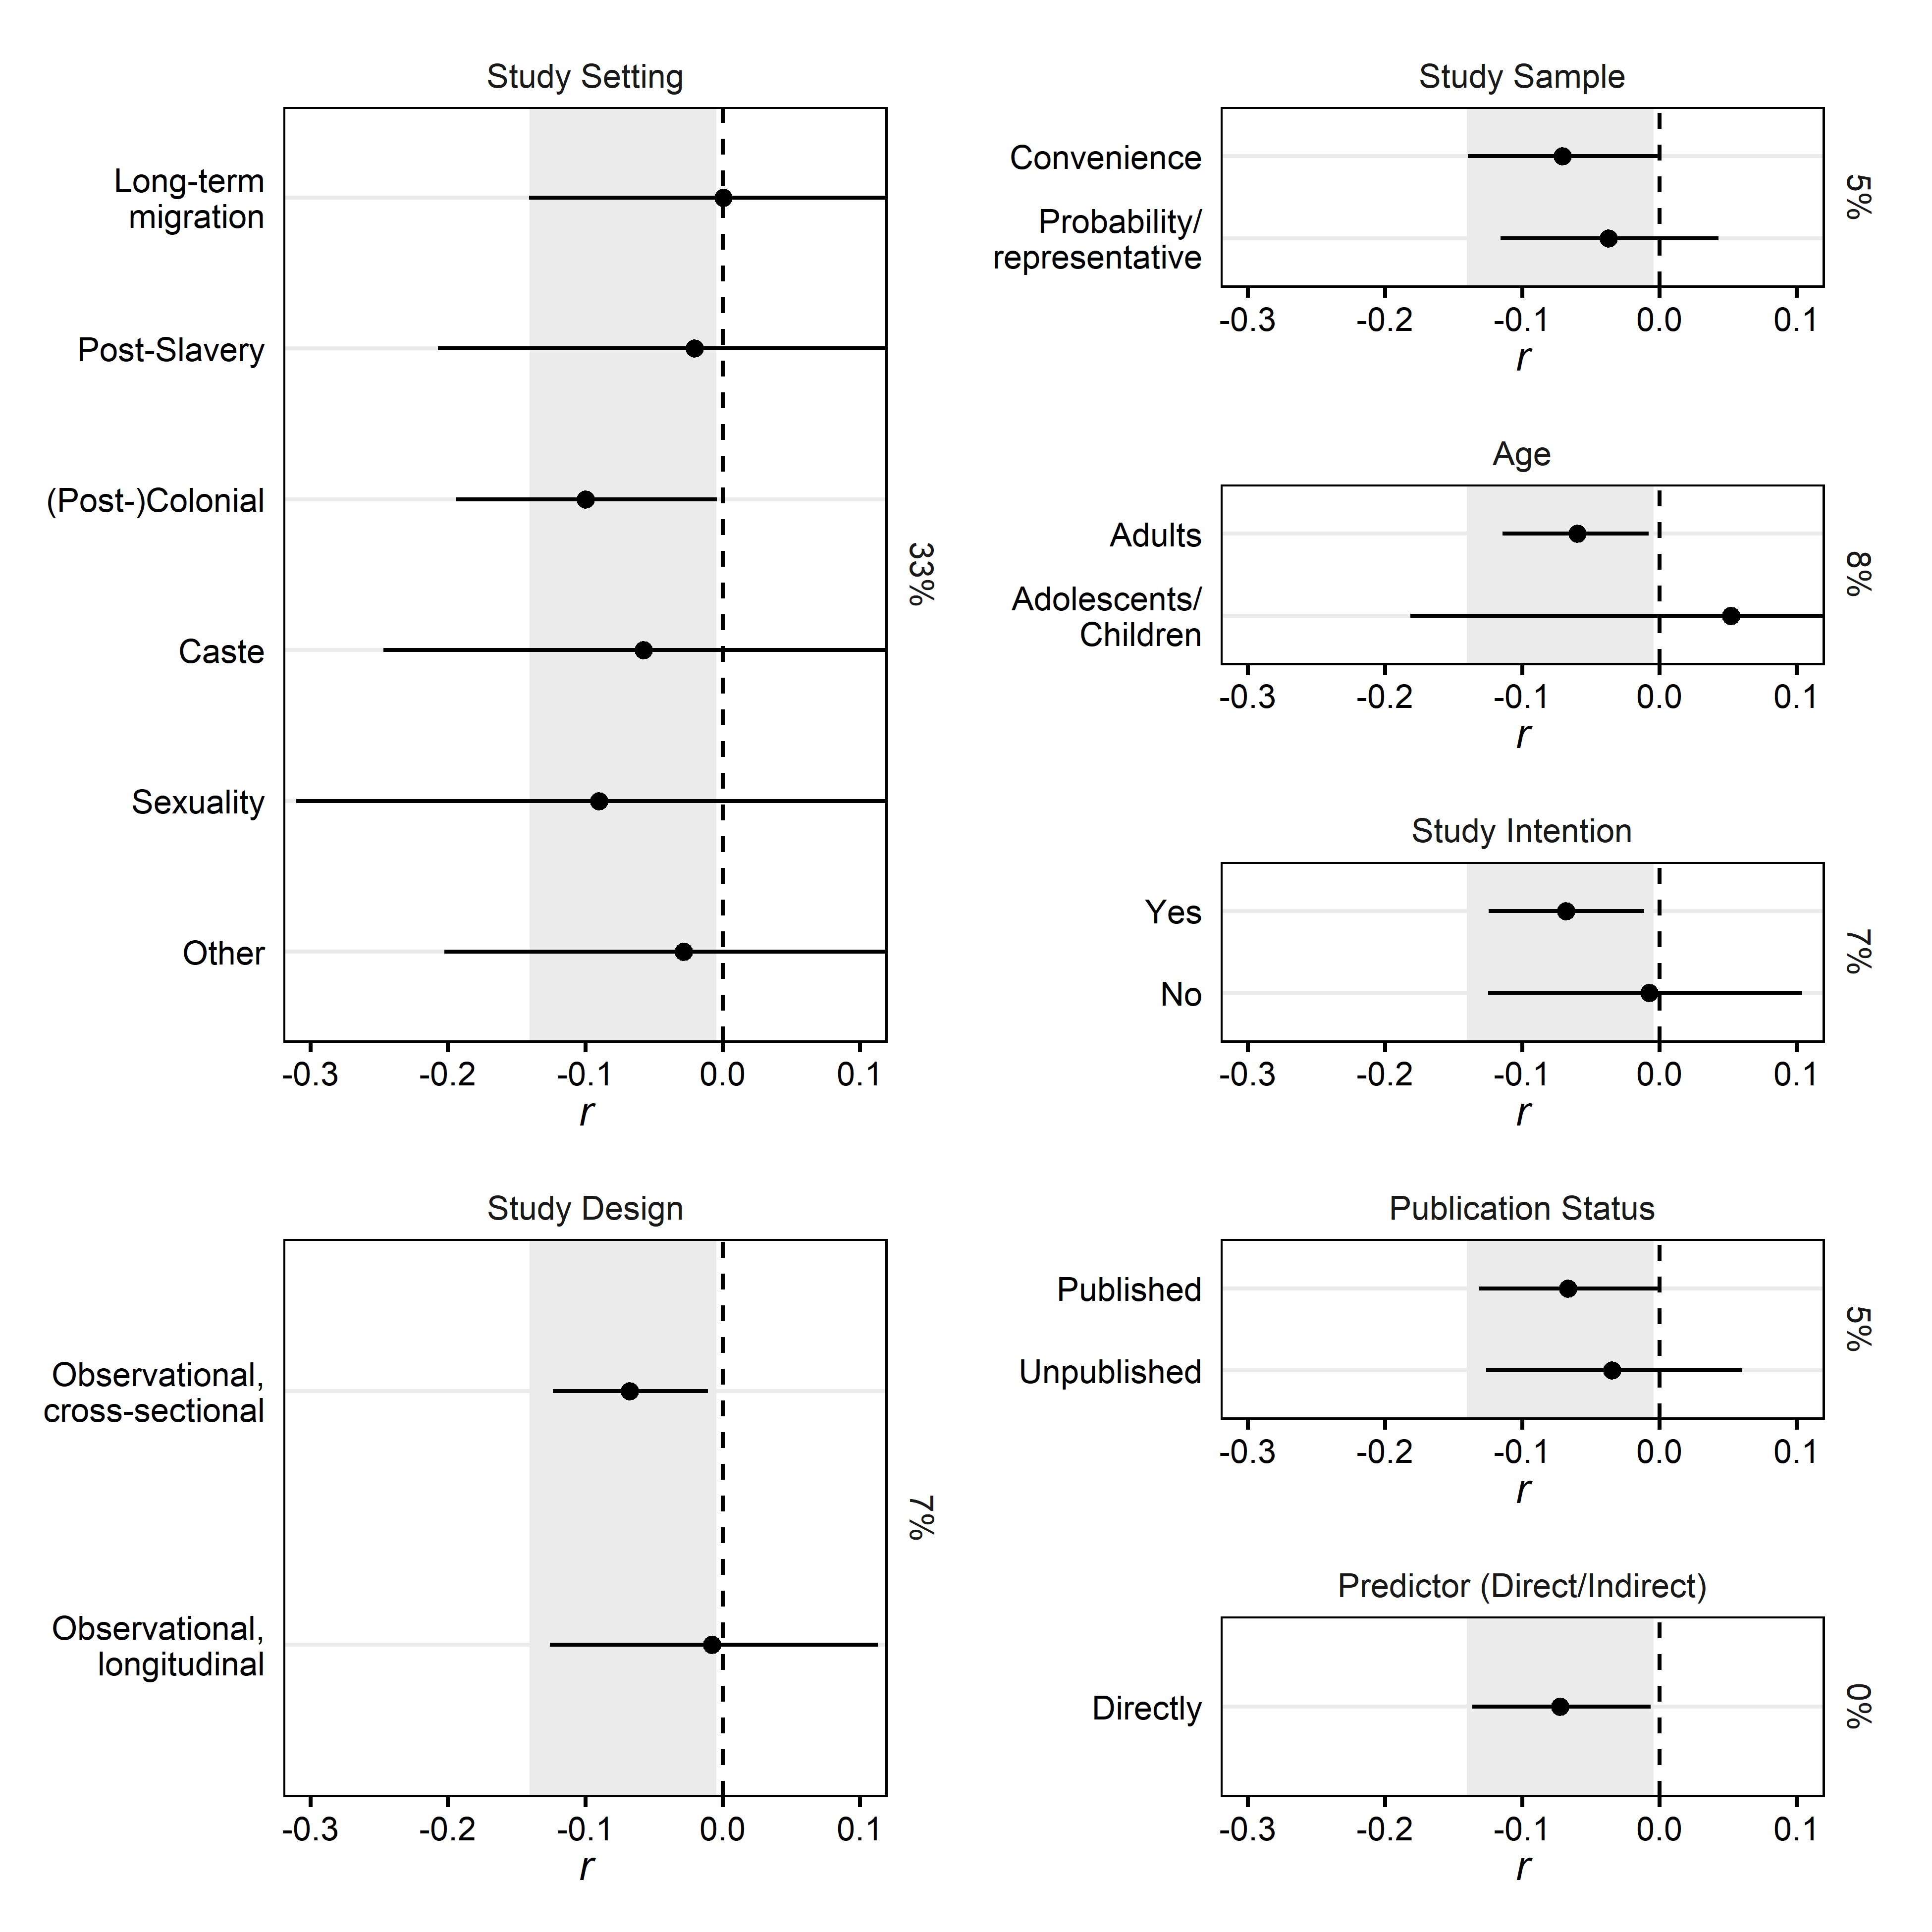
\includegraphics[scale=1]{../figures/figure-s2}
\caption*{\textit{Note.} Intervals enclose the 95\% most plausible estimates of the category-specific effect size. Shaded ribbons enclose the 95\% most plausible estimates of the mean effect size from the main analyses. Percentages indicate the estimated between-sample variance explained by each moderator variable.}
\label{fig:s2}
\end{figure*}

\hypertarget{moderator-analyses-without-contact-quality}{%
\subsection{Moderator Analyses Without Contact
Quality}\label{moderator-analyses-without-contact-quality}}

\begin{figure*}
\centering
\caption{Results from the random-effects meta-regression tree analysis}
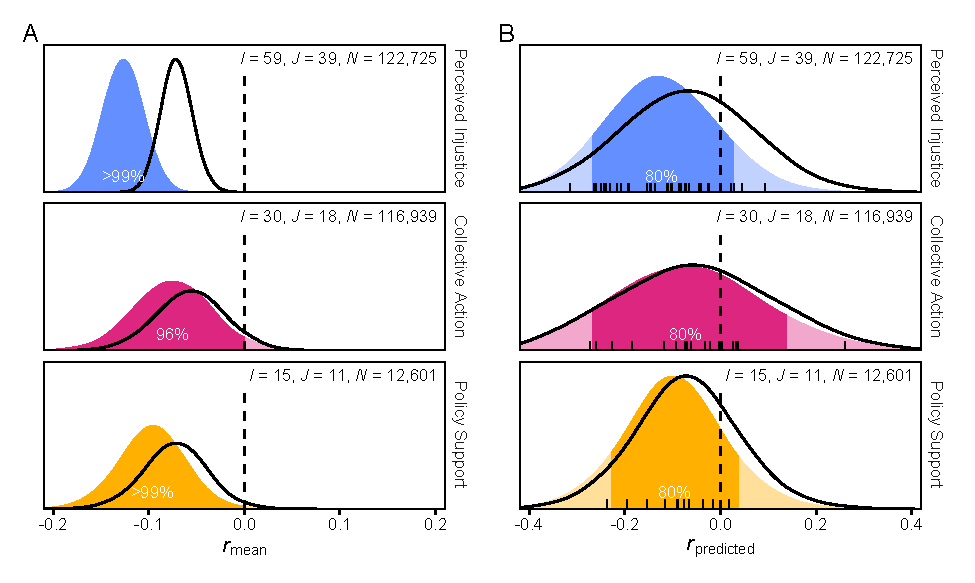
\includegraphics[scale=1]{../figures/figure-s3}
\caption*{\textit{Note.} Posterior distributions for the estimated correlation coefficient in each leaf of the meta-regression tree, highlighting the proportion of posterior samples for which $r_\text{mean} < 0$. In this analysis, we did not consider whether studies measured direct, qualitatively positive contact. S.-T. Migration = Short-Term Migration.}
\label{fig:s3}
\end{figure*}

In an earlier version of our manuscript, we did not consider the
distinction between contact quantity and quality as a moderator. As we
added this moderator during peer review and as doing so changed the
results of some of our moderator analyses, we report our original
findings from the moderator analyses below. We used meta-regression
trees to discover interactions between moderator variables that best
explained heterogeneity in effect sizes (Li et al., 2017, 2020). Figure
S3 shows the resulting meta-regression model, which explained more
variance across samples than any individual moderator (\(R^2 = 30\%\)).
We found that intergroup contact was associated with less perceived
injustice only in studies that focused on adults and that measured
intergroup contact directly. Among these studies, this association was
stronger in settings in which the groups' relative inequality stemmed
from short-term migration or colonization (\(r = -.18, [-.23, -.13]\))
than in other settings (\(r = -.09, [-.12, -.06]\)).

\hypertarget{unpublished-studies}{%
\subsection{Unpublished Studies}\label{unpublished-studies}}

Some of the unpublished data included in the meta-analysis were based on
studies that involved one of the co-authors of the present research. For
the sake of transparency, we describe each of these studies and refer to
published research based on these studies.

\textbf{Bracegirdle (2020)} is based on data from a longitudinal social
network study of two schools in a town in North West England conducted
by a graduate students who, at the time, was co-supervised by the first
author of the present research. The study included measures intended to
test a broad range of questions, for example, to disentangle how contact
and socialization effects shape outgroup attitudes in diverse friendship
networks (Bracegirdle et al., 2022). Bracegirdle (2020) includes data
from Asian adolescents who reported their cross-group friendships with
White adolescents (\emph{N} = 829).

\textbf{Schäfer et al. (2018)} is based on data from a longitudinal
survey of Asian British and White British people and included a broad
range of measures related to intergroup contact and intergroup relations
in England. Schäfer et al. (2018) includes data from Asian British
people who reported their contact experiences with White British people,
as well as their perceived discrimination and collective action
intentions (\emph{N} = 751).

\textbf{Sengupta (2020a)} and \textbf{Sengupta (2020b)} is based on data
from the Centre for the Monitoring of the Indian Economy's consumer
pyramid sample, a representative national sample of the Indian
population. In 2017, this sample consisted of 161,183 households
(112,657 rural and 48,526 urban households). Households were selected by
dividing 26 of the 29 States of India into sub-state ``Homogenous
Regions''---sets of neighboring districts with similar climatic
conditions and urbanization levels---and then randomly sampling
villages/blocks of towns, and households within each region. During
August and September, 2017, interviewers attempted to make face-to-face
contact with each household. One member of the household was asked to
volunteer to complete the verbally administered survey. In all, 134,531
people were successfully reached by interviewers. The survey included
measures intended to test a broad range of questions, for example, about
the relationship between ambivalent sexism and violence against women
(Sengupta, 2021). For the meta-analysis, we calculated correlation
coefficients between items measuring positive and negative contact,
group identification, perceived discrimination, and collective action
intentions. Items in the survey were first translated from English into
ten Indian languages (Hindi, Urdu, Marathi, Punjabi, Bengali, Tamil,
Telugu, Malayalam, Odiya and Gujarati), and then independently
back-translated to ensure accuracy. Surveys were administered in
whichever language the participants were most comfortable with
(including English). Sengupta (2020a) includes data from participants
who belonged to three disadvantaged caste groups and reported their
contact experiences with members of upper castes (\emph{N} = 96,547).
Sengupta (2020b) includes data from participants who belonged to four
religious minority groups and reported their contact experiences with
Hindus (\emph{N} = 7,440).

\textbf{Sengupta \& Sibley (2020)} is based on data from a large-scale
national longitudinal study in New Zealand, the New Zealand Attitudes
and Values Study (NZAVS;
\url{https://www.psych.auckland.ac.nz/en/about/new-zealand-attitudes-and-values-study.html}).
Sengupta \& Sibley (2020) includes data from Māori, Pacific Islanders,
and Asians who reported their contact experiences with European New
Zealanders (\emph{N} = 3187).

\textbf{Wölfer \& Hewstone (2019)} is based on data from a social
network study across ten schools in England which was conducted as part
of a project for which the first author of the present research worked
as a postdoctoral researcher. A survey company collected data from the
same grade (Year 10, equivalent to 9th grade in the US) at each school.
Data were collected between January and March 2018. Students completed a
pen-and-paper survey in a classroom session (40--45 minutes). As part of
a larger study on intergroup contact among young people, the survey
included items measuring cross-group friendship as well as perceptions
of discrimination. Wölfer \& Hewstone (2019) included data from Black,
Asian, and other ethnic minority students who reported their contact
experiences with White people (\emph{N} = 713).

\newpage

\hypertarget{references}{%
\section{References}\label{references}}

\begingroup

\noindent \setlength{\parindent}{-0.5in} \setlength{\leftskip}{0.5in}

\hypertarget{refs}{}
\begin{CSLReferences}{1}{0}
\leavevmode\hypertarget{ref-2398}{}%
*Bracegirdle, C. (2020). \emph{Social network study of two diverse
schools in {Northern England}} {[}Unpublished dataset{]}. University of
Oxford.

\leavevmode\hypertarget{ref-bracegirdle_disentangling_2022}{}%
Bracegirdle, C., Reimer, N. K., Zalk, M. van, Hewstone, M., \& Wölfer,
R. (2022). Disentangling contact and socialization effects on outgroup
attitudes in diverse friendship networks. \emph{Journal of Personality
and Social Psychology}, \emph{122}(1), 1--15.
\url{https://doi.org/10.1037/pspa0000240}

\leavevmode\hypertarget{ref-li_meta-cart_2017}{}%
Li, X., Dusseldorp, E., \& Meulman, J. J. (2017). Meta-{CART}: {A} tool
to identify interactions between moderators in meta-analysis.
\emph{British Journal of Mathematical and Statistical Psychology},
\emph{70}(1), 118--136. \url{https://doi.org/10.1111/bmsp.12088}

\leavevmode\hypertarget{ref-li_multiple_2020}{}%
Li, X., Dusseldorp, E., Su, X., \& Meulman, J. J. (2020). Multiple
moderator meta-analysis using the {R}-package {Meta}-{CART}.
\emph{Behavior Research Methods}, \emph{52}(6), 2657--2673.
\url{https://doi.org/10.3758/s13428-020-01360-0}

\leavevmode\hypertarget{ref-muthukrishna_beyond_2020}{}%
Muthukrishna, M., Bell, A. V., Henrich, J., Curtin, C. M., Gedranovich,
A., McInerney, J., \& Thue, B. (2020). Beyond western, educated,
industrial, rich, and democratic ({WEIRD}) psychology: Measuring and
mapping scales of cultural and psychological distance.
\emph{Psychological Science}, \emph{31}(6), 678--701.
\url{https://doi.org/10.1177/0956797620916782}

\leavevmode\hypertarget{ref-2382}{}%
*Schäfer, S. J., Bracegirdle, C., Christ, O., Hewstone, M., Jaspers, E.,
Reimer, N. K., \& Wölfer, R. (2018). \emph{Positive-negative asymmetry
of intergroup contact: A dynamic approach} {[}Unpublished dataset{]}.
University of Oxford.

\leavevmode\hypertarget{ref-2392}{}%
*Sengupta, N. K. (2020a). \emph{Inter-caste contact in {India}}
{[}Unpublished dataset{]}. University of Kent.

\leavevmode\hypertarget{ref-2385}{}%
*Sengupta, N. K. (2020b). \emph{Inter-religious contact in {India}}
{[}Unpublished dataset{]}. University of Kent.

\leavevmode\hypertarget{ref-sengupta_protect_unpublished}{}%
Sengupta, N. K. (2021). \emph{{``We protect, you serve''}: Ambivalent
sexism and violence against women in {India}} {[}Manuscript submitted
for publication{]}. School of Psychology, University of Kent.

\leavevmode\hypertarget{ref-2381}{}%
*Sengupta, N. K., \& Sibley, C. G. (2020). \emph{Intergroup contact and
political attitudes among ethnic minorities in {New Zealand}}
{[}Unpublished dataset{]}. The University of Auckland.

\leavevmode\hypertarget{ref-2383}{}%
*Wölfer, R., \& Hewstone, M. (2019). \emph{Social integration in diverse
societies: The importance of contact experiences in youth}
{[}Unpublished dataset{]}. University of Oxford.

\end{CSLReferences}

\endgroup

\end{document}